% GNUPLOT: LaTeX picture with Postscript
\documentclass{minimal}
% Set font size
\makeatletter
\def\@ptsize{1}
\InputIfFileExists{size11.clo}{}{%
   \GenericError{(gnuplot) \space\space\space\@spaces}{%
      Gnuplot Error: File `size11.clo' not found! Could not set font size%
   }{See the gnuplot documentation for explanation.%
   }{For using a font size a file `size<fontsize>.clo' has to exist.
        Falling back ^^Jto default fontsize 10pt.}%
  \def\@ptsize{0}
  \input{size10.clo}%
}%
\makeatother
% Load packages
\usepackage{calc}
\usepackage{graphicx}
\usepackage{color}
\usepackage{transparent}
\makeatletter
% Select an appropriate default driver (from TeXLive graphics.cfg)
\begingroup
  \chardef\x=0 %
  % check pdfTeX
  \@ifundefined{pdfoutput}{}{%
    \ifcase\pdfoutput
    \else
      \chardef\x=1 %
    \fi
  }%
  % check VTeX
  \@ifundefined{OpMode}{}{%
    \chardef\x=2 %
  }%
\expandafter\endgroup
\ifcase\x
  % default case
  \PassOptionsToPackage{dvips}{geometry}
\or
  % pdfTeX is running in pdf mode
  \PassOptionsToPackage{pdftex}{geometry}
\else
  % VTeX is running
  \PassOptionsToPackage{vtex}{geometry}
\fi
\makeatother
% Set papersize
\usepackage[papersize={566.00bp,1275.00bp},text={566.00bp,1275.00bp}]{geometry}
% No page numbers and no paragraph indentation
\pagestyle{empty}
\setlength{\parindent}{0bp}%
% Load configuration file
\InputIfFileExists{gnuplot.cfg}{%
  \typeout{Using configuration file gnuplot.cfg}%
}{%
 \typeout{No configuration file gnuplot.cfg found.}%
}%
%
\begin{document}
\begingroup
  \makeatletter
  \providecommand\color[2][]{%
    \GenericError{(gnuplot) \space\space\space\@spaces}{%
      Package color not loaded in conjunction with
      terminal option `colourtext'%
    }{See the gnuplot documentation for explanation.%
    }{Either use 'blacktext' in gnuplot or load the package
      color.sty in LaTeX.}%
    \renewcommand\color[2][]{}%
  }%
  \providecommand\includegraphics[2][]{%
    \GenericError{(gnuplot) \space\space\space\@spaces}{%
      Package graphicx or graphics not loaded%
    }{See the gnuplot documentation for explanation.%
    }{The gnuplot epslatex terminal needs graphicx.sty or graphics.sty.}%
    \renewcommand\includegraphics[2][]{}%
  }%
  \providecommand\rotatebox[2]{#2}%
  \@ifundefined{ifGPcolor}{%
    \newif\ifGPcolor
    \GPcolortrue
  }{}%
  \@ifundefined{ifGPblacktext}{%
    \newif\ifGPblacktext
    \GPblacktextfalse
  }{}%
  % define a \g@addto@macro without @ in the name:
  \let\gplgaddtomacro\g@addto@macro
  % define empty templates for all commands taking text:
  \gdef\gplbacktext{}%
  \gdef\gplfronttext{}%
  \makeatother
  \ifGPblacktext
    % no textcolor at all
    \def\colorrgb#1{}%
    \def\colorgray#1{}%
  \else
    % gray or color?
    \ifGPcolor
      \def\colorrgb#1{\color[rgb]{#1}}%
      \def\colorgray#1{\color[gray]{#1}}%
      \expandafter\def\csname LTw\endcsname{\color{white}}%
      \expandafter\def\csname LTb\endcsname{\color{black}}%
      \expandafter\def\csname LTa\endcsname{\color{black}}%
      \expandafter\def\csname LT0\endcsname{\color[rgb]{1,0,0}}%
      \expandafter\def\csname LT1\endcsname{\color[rgb]{0,1,0}}%
      \expandafter\def\csname LT2\endcsname{\color[rgb]{0,0,1}}%
      \expandafter\def\csname LT3\endcsname{\color[rgb]{1,0,1}}%
      \expandafter\def\csname LT4\endcsname{\color[rgb]{0,1,1}}%
      \expandafter\def\csname LT5\endcsname{\color[rgb]{1,1,0}}%
      \expandafter\def\csname LT6\endcsname{\color[rgb]{0,0,0}}%
      \expandafter\def\csname LT7\endcsname{\color[rgb]{1,0.3,0}}%
      \expandafter\def\csname LT8\endcsname{\color[rgb]{0.5,0.5,0.5}}%
    \else
      % gray
      \def\colorrgb#1{\color{black}}%
      \def\colorgray#1{\color[gray]{#1}}%
      \expandafter\def\csname LTw\endcsname{\color{white}}%
      \expandafter\def\csname LTb\endcsname{\color{black}}%
      \expandafter\def\csname LTa\endcsname{\color{black}}%
      \expandafter\def\csname LT0\endcsname{\color{black}}%
      \expandafter\def\csname LT1\endcsname{\color{black}}%
      \expandafter\def\csname LT2\endcsname{\color{black}}%
      \expandafter\def\csname LT3\endcsname{\color{black}}%
      \expandafter\def\csname LT4\endcsname{\color{black}}%
      \expandafter\def\csname LT5\endcsname{\color{black}}%
      \expandafter\def\csname LT6\endcsname{\color{black}}%
      \expandafter\def\csname LT7\endcsname{\color{black}}%
      \expandafter\def\csname LT8\endcsname{\color{black}}%
    \fi
  \fi
    \setlength{\unitlength}{0.0500bp}%
    \ifx\gptboxheight\undefined%
      \newlength{\gptboxheight}%
      \newlength{\gptboxwidth}%
      \newsavebox{\gptboxtext}%
    \fi%
    \setlength{\fboxrule}{0.5pt}%
    \setlength{\fboxsep}{1pt}%
\begin{picture}(11320.00,25500.00)%
    \gplgaddtomacro\gplbacktext{%
      \csname LTb\endcsname%%
      \put(1256,17595){\makebox(0,0)[r]{\strut{}$0$}}%
      \csname LTb\endcsname%%
      \put(1256,18309){\makebox(0,0)[r]{\strut{}$500$}}%
      \csname LTb\endcsname%%
      \put(1256,19023){\makebox(0,0)[r]{\strut{}$1000$}}%
      \csname LTb\endcsname%%
      \put(1256,19737){\makebox(0,0)[r]{\strut{}$1500$}}%
      \csname LTb\endcsname%%
      \put(1256,20451){\makebox(0,0)[r]{\strut{}$2000$}}%
      \csname LTb\endcsname%%
      \put(1256,21165){\makebox(0,0)[r]{\strut{}$2500$}}%
      \csname LTb\endcsname%%
      \put(1256,21878){\makebox(0,0)[r]{\strut{}$3000$}}%
      \csname LTb\endcsname%%
      \put(1256,22592){\makebox(0,0)[r]{\strut{}$3500$}}%
      \csname LTb\endcsname%%
      \put(1256,23306){\makebox(0,0)[r]{\strut{}$4000$}}%
      \csname LTb\endcsname%%
      \put(1256,24020){\makebox(0,0)[r]{\strut{}$4500$}}%
      \csname LTb\endcsname%%
      \put(1256,24734){\makebox(0,0)[r]{\strut{}$5000$}}%
      \csname LTb\endcsname%%
      \put(1358,17409){\makebox(0,0){\strut{}$-10$}}%
      \csname LTb\endcsname%%
      \put(2298,17409){\makebox(0,0){\strut{}$-8$}}%
      \csname LTb\endcsname%%
      \put(3237,17409){\makebox(0,0){\strut{}$-6$}}%
      \csname LTb\endcsname%%
      \put(4177,17409){\makebox(0,0){\strut{}$-4$}}%
      \csname LTb\endcsname%%
      \put(5116,17409){\makebox(0,0){\strut{}$-2$}}%
      \csname LTb\endcsname%%
      \put(6056,17409){\makebox(0,0){\strut{}$0$}}%
      \csname LTb\endcsname%%
      \put(6995,17409){\makebox(0,0){\strut{}$2$}}%
      \csname LTb\endcsname%%
      \put(7935,17409){\makebox(0,0){\strut{}$4$}}%
      \csname LTb\endcsname%%
      \put(8874,17409){\makebox(0,0){\strut{}$6$}}%
      \csname LTb\endcsname%%
      \put(9814,17409){\makebox(0,0){\strut{}$8$}}%
      \csname LTb\endcsname%%
      \put(10753,17409){\makebox(0,0){\strut{}$10$}}%
    }%
    \gplgaddtomacro\gplfronttext{%
      \csname LTb\endcsname%%
      \put(458,21164){\rotatebox{-270}{\makebox(0,0){\strut{}\Huge Frequency}}}%
      \csname LTb\endcsname%%
      \put(6055,16944){\makebox(0,0){\strut{}\Huge$x$}}%
      \csname LTb\endcsname%%
      \put(9965,24567){\makebox(0,0)[r]{\strut{}Simulation}}%
      \csname LTb\endcsname%%
      \put(9965,24381){\makebox(0,0)[r]{\strut{}Theory}}%
      \csname LTb\endcsname%%
      \put(1640,24163){\makebox(0,0)[l]{\strut{}\huge$\mu=0,\sigma=1$}}%
    }%
    \gplgaddtomacro\gplbacktext{%
      \csname LTb\endcsname%%
      \put(1256,9180){\makebox(0,0)[r]{\strut{}$0$}}%
      \csname LTb\endcsname%%
      \put(1256,10200){\makebox(0,0)[r]{\strut{}$2000$}}%
      \csname LTb\endcsname%%
      \put(1256,11220){\makebox(0,0)[r]{\strut{}$4000$}}%
      \csname LTb\endcsname%%
      \put(1256,12240){\makebox(0,0)[r]{\strut{}$6000$}}%
      \csname LTb\endcsname%%
      \put(1256,13259){\makebox(0,0)[r]{\strut{}$8000$}}%
      \csname LTb\endcsname%%
      \put(1256,14279){\makebox(0,0)[r]{\strut{}$10000$}}%
      \csname LTb\endcsname%%
      \put(1256,15299){\makebox(0,0)[r]{\strut{}$12000$}}%
      \csname LTb\endcsname%%
      \put(1256,16319){\makebox(0,0)[r]{\strut{}$14000$}}%
      \csname LTb\endcsname%%
      \put(1358,8994){\makebox(0,0){\strut{}$-10$}}%
      \csname LTb\endcsname%%
      \put(2298,8994){\makebox(0,0){\strut{}$-8$}}%
      \csname LTb\endcsname%%
      \put(3237,8994){\makebox(0,0){\strut{}$-6$}}%
      \csname LTb\endcsname%%
      \put(4177,8994){\makebox(0,0){\strut{}$-4$}}%
      \csname LTb\endcsname%%
      \put(5116,8994){\makebox(0,0){\strut{}$-2$}}%
      \csname LTb\endcsname%%
      \put(6056,8994){\makebox(0,0){\strut{}$0$}}%
      \csname LTb\endcsname%%
      \put(6995,8994){\makebox(0,0){\strut{}$2$}}%
      \csname LTb\endcsname%%
      \put(7935,8994){\makebox(0,0){\strut{}$4$}}%
      \csname LTb\endcsname%%
      \put(8874,8994){\makebox(0,0){\strut{}$6$}}%
      \csname LTb\endcsname%%
      \put(9814,8994){\makebox(0,0){\strut{}$8$}}%
      \csname LTb\endcsname%%
      \put(10753,8994){\makebox(0,0){\strut{}$10$}}%
    }%
    \gplgaddtomacro\gplfronttext{%
      \csname LTb\endcsname%%
      \put(356,12749){\rotatebox{-270}{\makebox(0,0){\strut{}\Huge Frequency}}}%
      \csname LTb\endcsname%%
      \put(6055,8529){\makebox(0,0){\strut{}\Huge$x$}}%
      \csname LTb\endcsname%%
      \put(9965,16152){\makebox(0,0)[r]{\strut{}Simulation}}%
      \csname LTb\endcsname%%
      \put(9965,15966){\makebox(0,0)[r]{\strut{}Theory}}%
      \csname LTb\endcsname%%
      \put(1640,15748){\makebox(0,0)[l]{\strut{}\huge$\mu=\pm2,\sigma=1$}}%
    }%
    \gplgaddtomacro\gplbacktext{%
      \csname LTb\endcsname%%
      \put(1256,765){\makebox(0,0)[r]{\strut{}$0$}}%
      \csname LTb\endcsname%%
      \put(1256,1479){\makebox(0,0)[r]{\strut{}$1000$}}%
      \csname LTb\endcsname%%
      \put(1256,2193){\makebox(0,0)[r]{\strut{}$2000$}}%
      \csname LTb\endcsname%%
      \put(1256,2907){\makebox(0,0)[r]{\strut{}$3000$}}%
      \csname LTb\endcsname%%
      \put(1256,3621){\makebox(0,0)[r]{\strut{}$4000$}}%
      \csname LTb\endcsname%%
      \put(1256,4335){\makebox(0,0)[r]{\strut{}$5000$}}%
      \csname LTb\endcsname%%
      \put(1256,5048){\makebox(0,0)[r]{\strut{}$6000$}}%
      \csname LTb\endcsname%%
      \put(1256,5762){\makebox(0,0)[r]{\strut{}$7000$}}%
      \csname LTb\endcsname%%
      \put(1256,6476){\makebox(0,0)[r]{\strut{}$8000$}}%
      \csname LTb\endcsname%%
      \put(1256,7190){\makebox(0,0)[r]{\strut{}$9000$}}%
      \csname LTb\endcsname%%
      \put(1256,7904){\makebox(0,0)[r]{\strut{}$10000$}}%
      \csname LTb\endcsname%%
      \put(1358,579){\makebox(0,0){\strut{}$-10$}}%
      \csname LTb\endcsname%%
      \put(2298,579){\makebox(0,0){\strut{}$-8$}}%
      \csname LTb\endcsname%%
      \put(3237,579){\makebox(0,0){\strut{}$-6$}}%
      \csname LTb\endcsname%%
      \put(4177,579){\makebox(0,0){\strut{}$-4$}}%
      \csname LTb\endcsname%%
      \put(5116,579){\makebox(0,0){\strut{}$-2$}}%
      \csname LTb\endcsname%%
      \put(6056,579){\makebox(0,0){\strut{}$0$}}%
      \csname LTb\endcsname%%
      \put(6995,579){\makebox(0,0){\strut{}$2$}}%
      \csname LTb\endcsname%%
      \put(7935,579){\makebox(0,0){\strut{}$4$}}%
      \csname LTb\endcsname%%
      \put(8874,579){\makebox(0,0){\strut{}$6$}}%
      \csname LTb\endcsname%%
      \put(9814,579){\makebox(0,0){\strut{}$8$}}%
      \csname LTb\endcsname%%
      \put(10753,579){\makebox(0,0){\strut{}$10$}}%
    }%
    \gplgaddtomacro\gplfronttext{%
      \csname LTb\endcsname%%
      \put(356,4334){\rotatebox{-270}{\makebox(0,0){\strut{}\Huge Frequency}}}%
      \csname LTb\endcsname%%
      \put(6055,114){\makebox(0,0){\strut{}\Huge$x$}}%
      \csname LTb\endcsname%%
      \put(9965,7737){\makebox(0,0)[r]{\strut{}Simulation}}%
      \csname LTb\endcsname%%
      \put(9965,7551){\makebox(0,0)[r]{\strut{}Theory}}%
      \csname LTb\endcsname%%
      \put(1640,7333){\makebox(0,0)[l]{\strut{}\huge$\mu=\left\{-5,0,5\right\}$}}%
      \csname LTb\endcsname%%
      \put(1640,6619){\makebox(0,0)[l]{\strut{}\huge$\sigma=\left\{1,1,1\right\}$}}%
    }%
    \gplbacktext
    \put(0,0){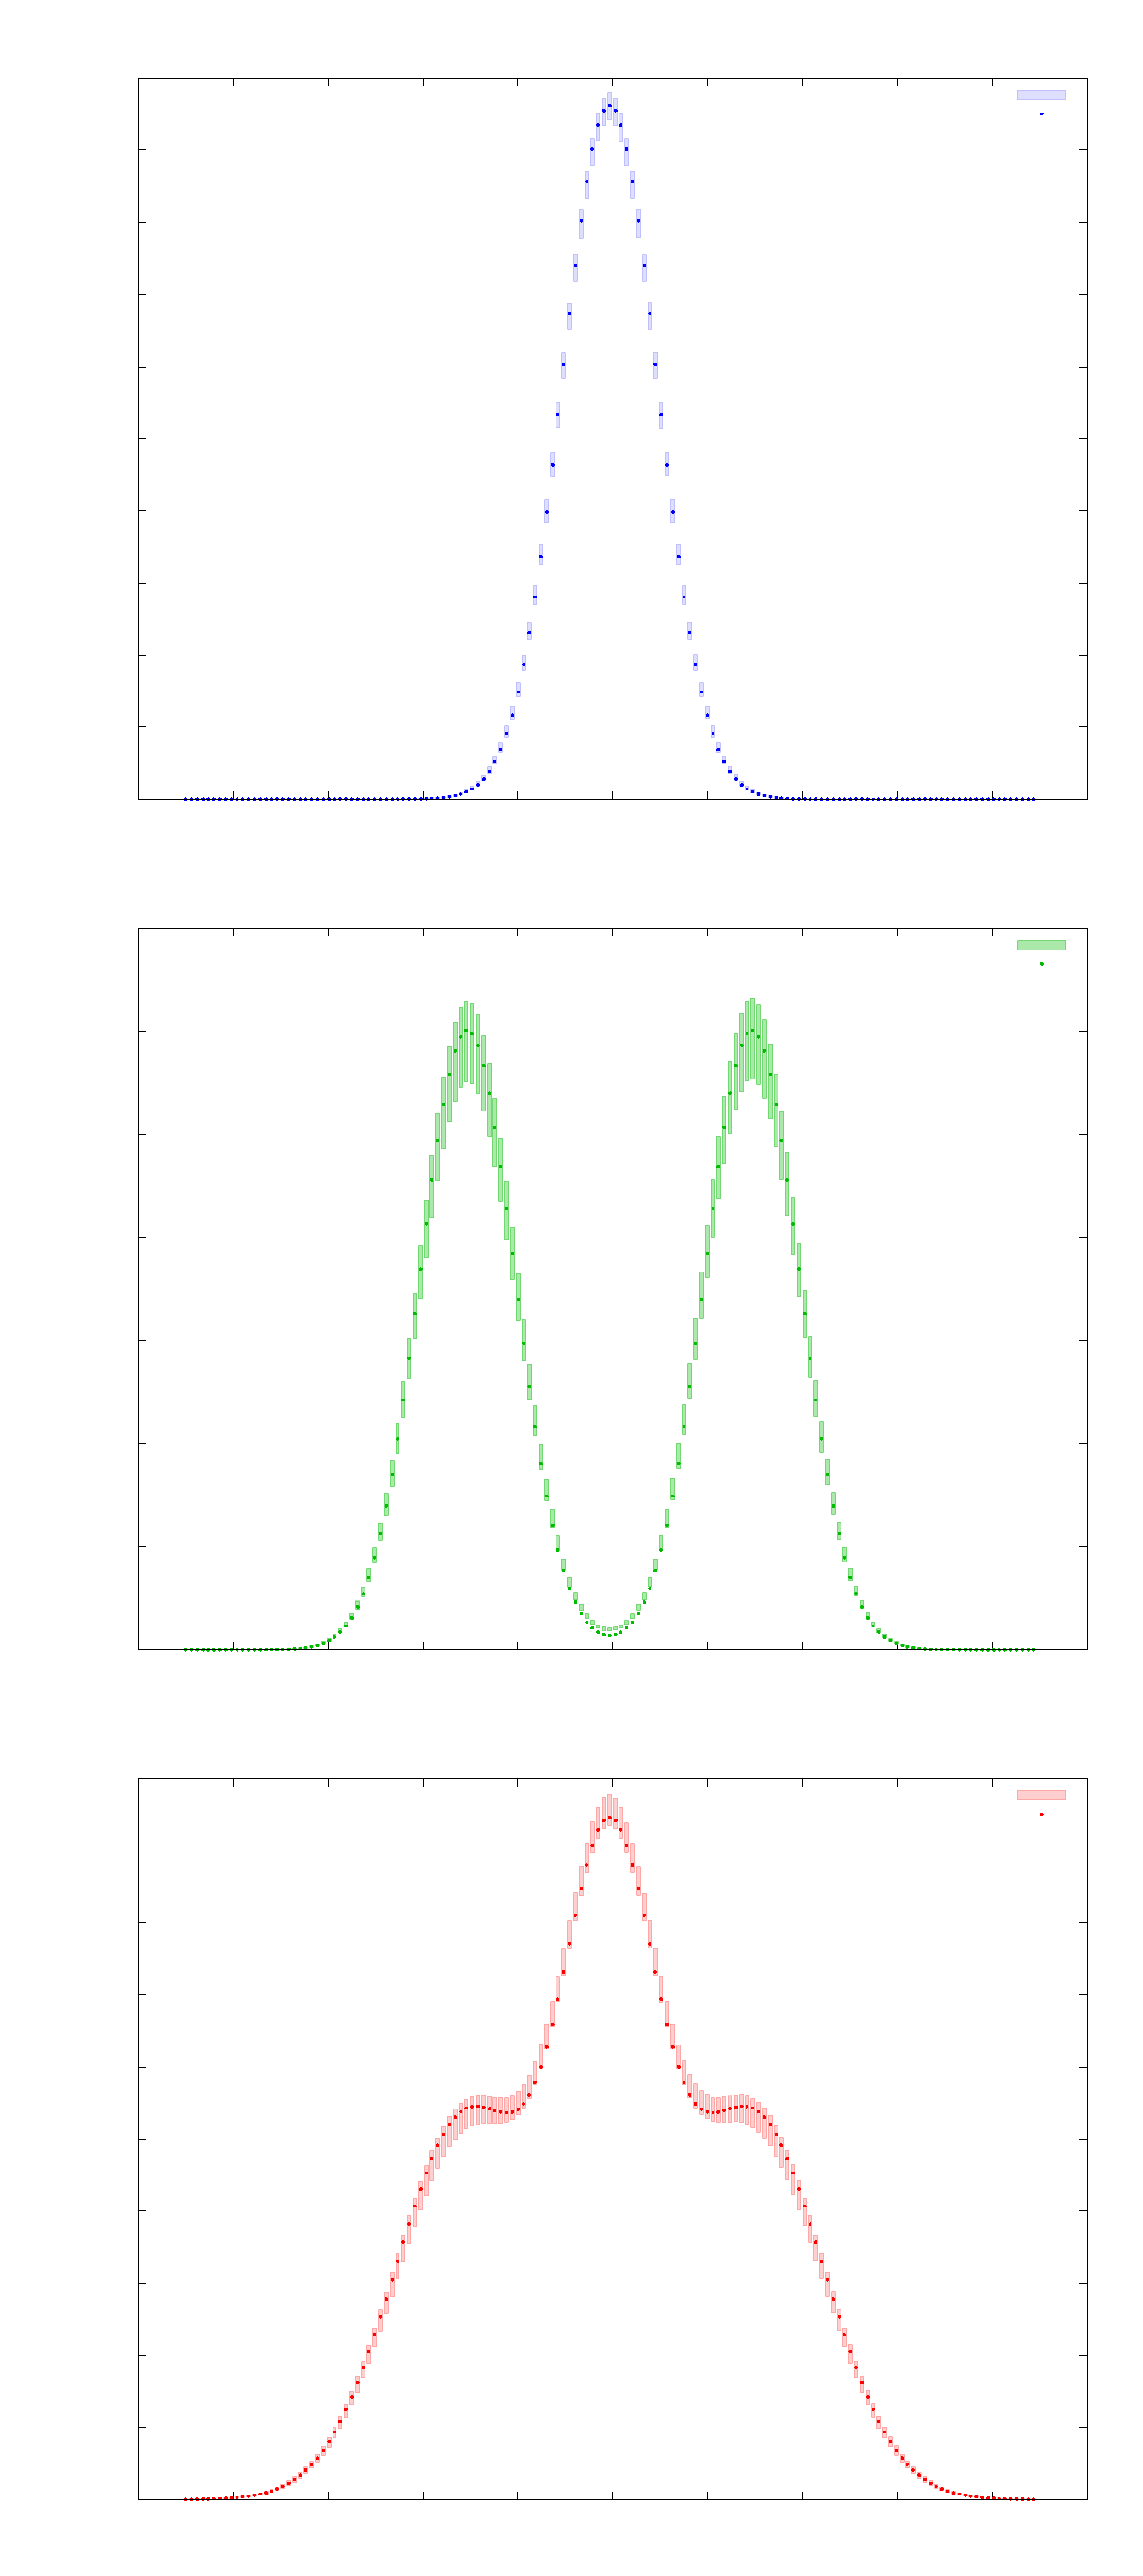
\includegraphics{plot-inc}}%
    \gplfronttext
  \end{picture}%
\endgroup
\end{document}
